\begin{figure}[!t]
{\subfloat[Horizontal representation of $\mathcal{D}$]{
\label{back_horizontalexampledataset}
\begin{tabular}{|c|l|}
\hline
\multicolumn{2}{|c|}{$\mathcal{D}$}\\
\hline
\hline
	tid & items \\
\hline
	1 &	a b c d \\
\hline
2 &	a c d e\\
\hline
	3 &b c d e\\
\hline
4 &	a d e \\
\hline
\end{tabular}}}
\hfil
{\subfloat[Transposed representation of $\mathcal{D}$]{
\label{back_TTexampledataset}
\begin{tabular}{|c|l|}

\hline
\multicolumn{2}{|c|}{$TT$}\\
\hline
\hline
	item & tidlist \\ \hline
	a & 1,2,4 \\ \hline
	b & 1,3 \\ \hline
	c & 1,2,3 \\ \hline
	d & 1,2,3,4 \\ \hline
	e & 2,3,4 \\ \hline
\end{tabular}}}%
\hfil
{\subfloat[Frequent itemset extracted from $\mathcal{D}$ with a minsup=2 ]{
\label{back_frequent}
\begin{tabular}{|c|l|}
\hline
\multicolumn{2}{|c|}{Frequent itemsets}\\
\hline
\hline
itemset & support \\
\hline
a & 3\\
\hline
b & 2 \\
\hline
c & 3\\
\hline
d & 4\\
\hline
e& 3 \\ 
\hline
	a c & 2\\
\hline
	a d & 3\\
\hline
	a e & 2\\
\hline
	b c & 2\\
\hline
b d & 2\\
\hline
	c d & 3\\
\hline
	c e & 2\\
\hline
	d e & 3\\
\hline
a c d & 2\\
\hline
a d e& 2\\
\hline
b c d & 2\\
\hline
c d e & 2\\
\hline
\end{tabular}}}%
\caption{Running example dataset $\mathcal{D}$}
\label{back_exampledataset}
\end{figure}

A frequent itemset represents frequently  co-occurring items in a transactional dataset. 
More formally, let $\mathcal{I}$ be a set of items. A transactional dataset $\mathcal{D}$
consists of a set of transactions $\{t_1, \dots, t_n\}$.
Each transaction $t_i\in \mathcal{D}$ is a collection of items
(i.e., $t_i\subseteq \mathcal{I}$)
and is identified by a transaction identifier ($tid_i$).
Figure~\ref{back_horizontalexampledataset} reports an example of a transactional
dataset with 4 transactions.


An itemset $I$ is defined as a set of items (i.e., $I\subseteq\mathcal{I}$)
and is characterized by a support value, which is denoted by $sup(I)$ and
defined as the ratio between the number of transactions in $\mathcal{D}$
containing $I$ and the total number of transactions in $\mathcal{D}$.
In the example dataset in Figure~\ref{back_horizontalexampledataset}, for example,
the support of the itemset \textit{\{a,c,d\}} is 50\% (2/4). This value represents the frequency of occurrence of the itemset in the dataset. An itemset $I$ is considered frequent if its support is greater than a
user-provided minimum support threshold $minsup$. Figure~\ref{back_frequent}
reports the frequent itemset extracted from $\mathcal{D}$ with a minsup value equal to 50\% (i.e., an absolute support equal to 2).

Given a transactional dataset $\mathcal{D}$ and a minimum support
threshold $minsup$, the Frequent Itemset Mining \cite{SurveyHan2007} problem
consists in extracting the complete set of frequent itemsets
from $\mathcal{D}$.

The dimension of the search space can be represented as a lattice, whose top is an empty set. Its size increases exponentially with the number of items~\cite{goethals2003survey}.
In Figure~\ref{lattice}, the lattice related to our running example is shown.

\begin{figure}[!t]
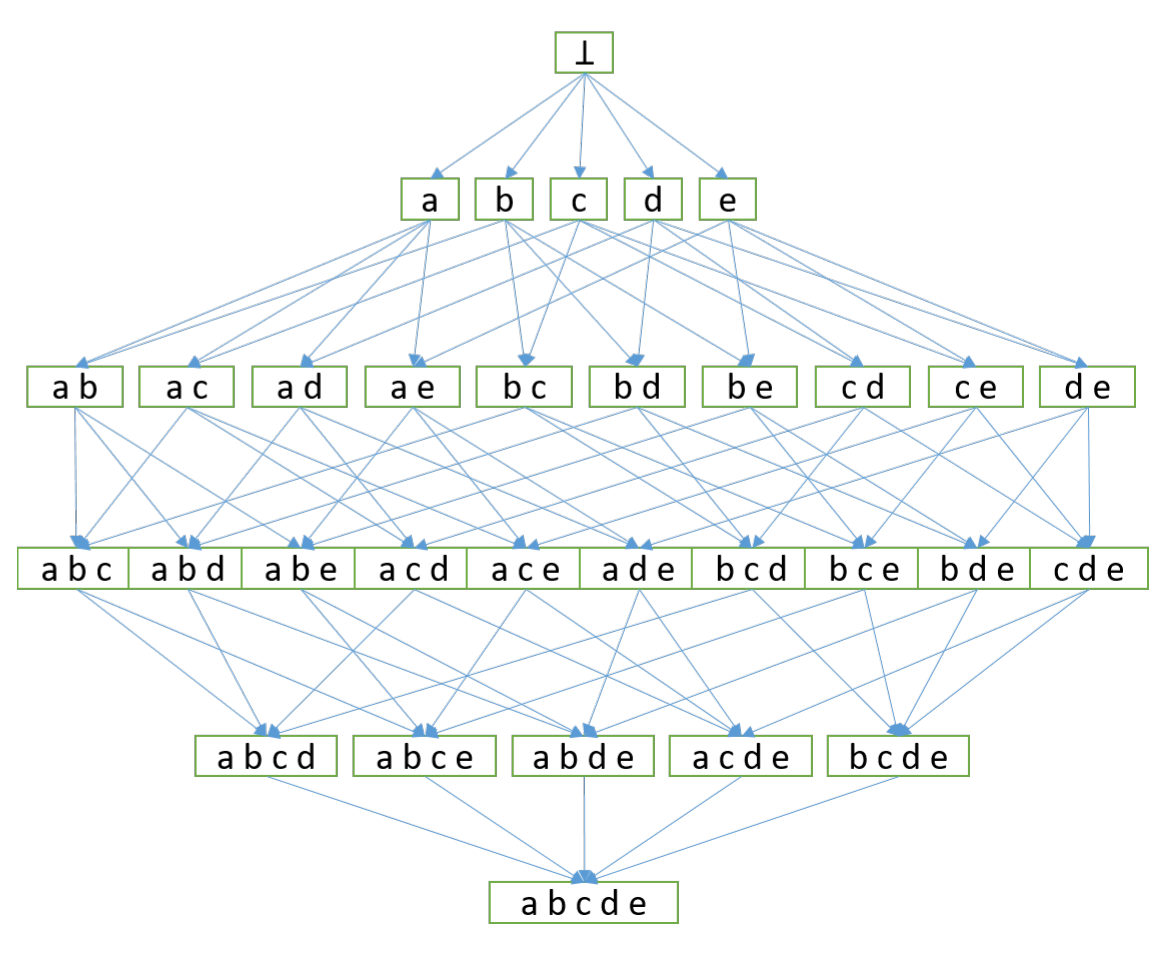
\includegraphics[width=5in]{immagini/lattices.eps}
\caption{Lattice representing the search space based on the items appearing in the example dataset $\mathcal{D}$}
\label{lattice}
\end{figure}


In this paper, we focus on closed itemsets.
Closed itemsets~\cite{ClosedPasquier1999} are a
particular and valuable subset of frequent itemsets, being
a concise but complete representation of the set of frequent itemsets. 
Precisely, an itemset $I$ is closed if none of its supersets (i.e. the set of itemsets which include $I$) has the same support count as $I$. For instance, in our running example, given a $minsup=2$, the itemset \textit{\{a,d\}} is a closed frequent itemset (support=3). The itemset \textit{\{a,c\}}, instead, is a frequent itemset (support=2), but it is not closed because of the presence of the itemset \textit{\{a,c,d\}} (support=2). 

A transactional dataset can also be represented in a vertical format, in which each
row represents an item $i$ and the list of tids of the transactions in which it appears,
also called $tidlist(\{i\})$.
For instance, the tidlist of the item \textit{a} in
the example dataset $\mathcal{D}$ is $\{1,2,4\}$.
Figure~\ref{back_TTexampledataset} reports the transposed representation of the
running example reported in Figure~\ref{back_horizontalexampledataset}. The main
advantage of the vertical format is the possibility to obtain the tidlist of
an itemset by intersecting the tidlists of the included items, without the
need of a full scan of the dataset.






